\documentclass[11pt]{report}
\usepackage{graphicx, subfigure}
\usepackage{mathtools}
\usepackage{hyperref}
\usepackage{float}
\usepackage[section]{placeins}
\usepackage{listings}

\lstset{frame=tb,
    language=Python,
    basicstyle={\small\ttfamily},
    breaklines=true,
    breakatwhitespace=true,
    tabsize=3
}

\begin{document}

    \title{Molecular Dynamics Calculaions for Multiscale Materials Modeling}
    \author{Bruce Berry}
    \maketitle

    \section{Introduction}
    This report details the simulation of various molecular scale events.  The Molecular Dynamics (MD) method is used to simulate inter-particle interactions.

    \section{Background}
    Molecular Dynamics methods treat the interactions of individial atoms in a lattice to determine the behavior of a material on the atomic scale.  Atoms are arranged on a lattice representing the initial structure of the model.  The positions of the atoms are updated according to forces that result from the potentials chosen for the problem at hand.  By studying the changing structure of the atoms, a material's response to external forces can be understood.

    \section{Methods}
        \subsection{Copper Nanowire}
        \begin{figure}[!htb]
            \label{fig:applied-stress-partA}
            \centering
            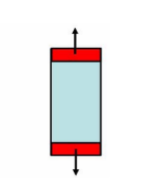
\includegraphics[width=0.4\textwidth]{applied-stress-partA.png}
            \caption{The stress Initial Condition.}
        \end{figure}
        Of interest is the simulation of a copper Nanowire's reponse to deformation.  Simulations were carried out using Nanohub's Nanowire Tensile Deformation Lab (NTDL) module.  A lattice of atoms was generated of size 20 x 20 x 130 \AA. As per the assignment's direction, the NTDL parameters were set to 8 x 8 x 36 to produce this initial condition.  The structure was set to be a free surface in each direction, with a tensile force applied to each end ~\ref{fig:applied-stress-partA}.  The tensile stress was implemented by applying a displacement of 0.02 \AA every 20 simulation time steps. 30,000 time steps were performed.  The simulation was carried out a second time, with the cross sectional area doubled (40 x 40 x 130 \AA).

        \subsection{Collagen Stretching}
        \begin{figure}[!htb]
            \label{fig:applied-stress-partB}
            \centering
            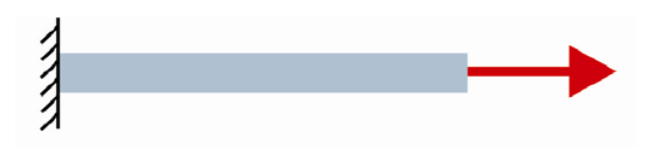
\includegraphics[width=0.4\textwidth]{applied-stress-partB.png}
            \caption{The stress initial condition.}
        \end{figure}
        To be investigated is the behavior of a collagen analog when subjected to a tensile force.  The software used the package Stretching Simulation of an Alpha-Helical Protein Domain (SSAPD).  SSAPD uses the method of Steered Molecular Dynamics (SMD) with a CHARMM force field to simulate the interaction of the molecule's componenets.  The boundary conditions are those indicated in ~\ref{fig:applied-stress-partB}.  Molecule data, including initial positions of atoms, points of fixation, and force field potentials were provided.  The SSAPD module was given the parameters according to:\\
        \\
        \begin{tabular}[!htb]{|c|c|c|c|}
            \hline
            DCD Freq. & Velocity & Steps & Averaging Bins \\
            \hline
            150 & 0.0005 & 150,000 & 300 \\
            \hline
        \end{tabular}

    \section{Results}

        \subsection{Copper Nanowire}
        \begin{figure}
            \label{fig:stress-small-fit}
            \centering
            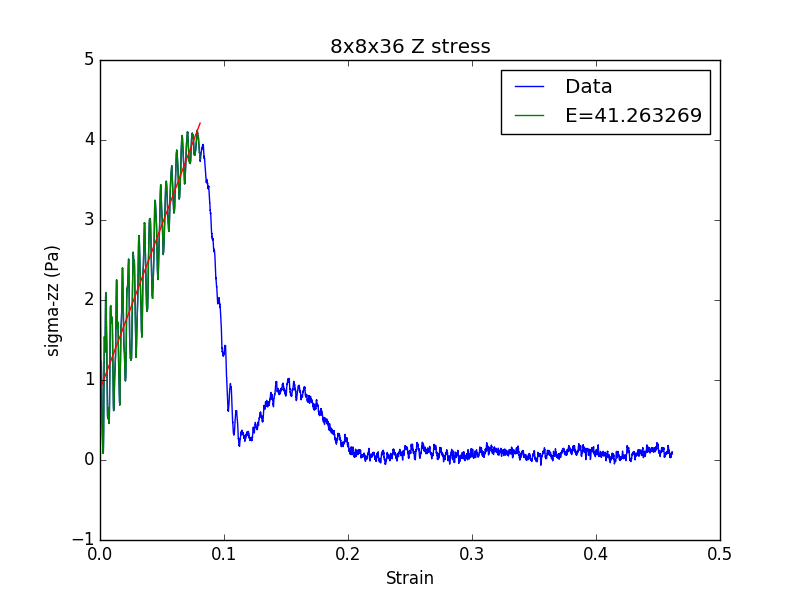
\includegraphics[width=0.4\textwidth]{sigma33-small-fit.png}
            \caption{Fit for 8x8x46 nanowire.}
        \end{figure}
        \begin{figure}
            \label{fig:stress-large-fit}
            \centering
            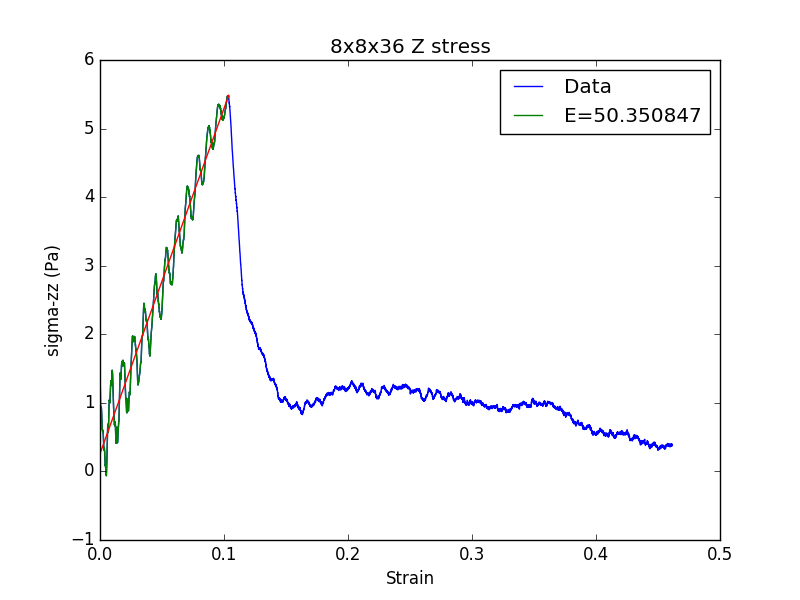
\includegraphics[width=0.4\textwidth]{sigma33-large-fit.png}
            \caption{Fit for 16x16x46 nanowire.}
        \end{figure}
        \begin{figure}
            \label{fig:rawdata-small}
            \centering
            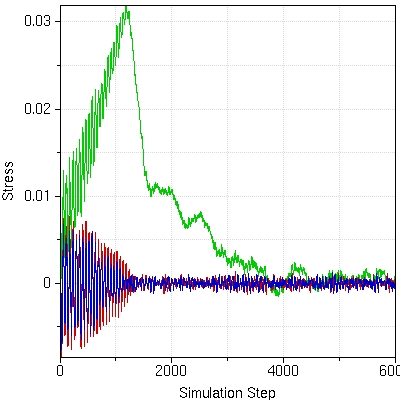
\includegraphics[width=0.4\textwidth]{StressvsSimulationStep-small.jpg}
            \caption{Stress tensor for 8x8x16 nanowire. Step size is sim-step*5.}
        \end{figure}
        \begin{figure}
            \label{fig:rawdata-large}
            \centering
            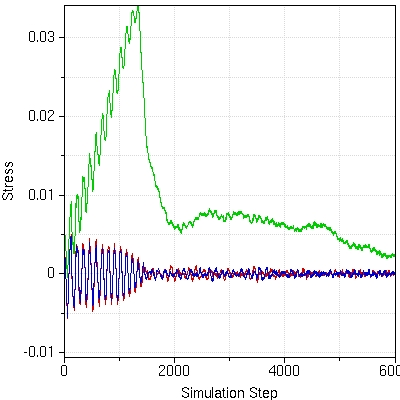
\includegraphics[width=0.4\textwidth]{StressvsSimulationStep-large.jpg}
            \caption{Stress tensor for 16x16x36 nanowire.Step size is sim-step*5.}
        \end{figure}
        \begin{figure}
            \label{fig:evolution}
            \centering
            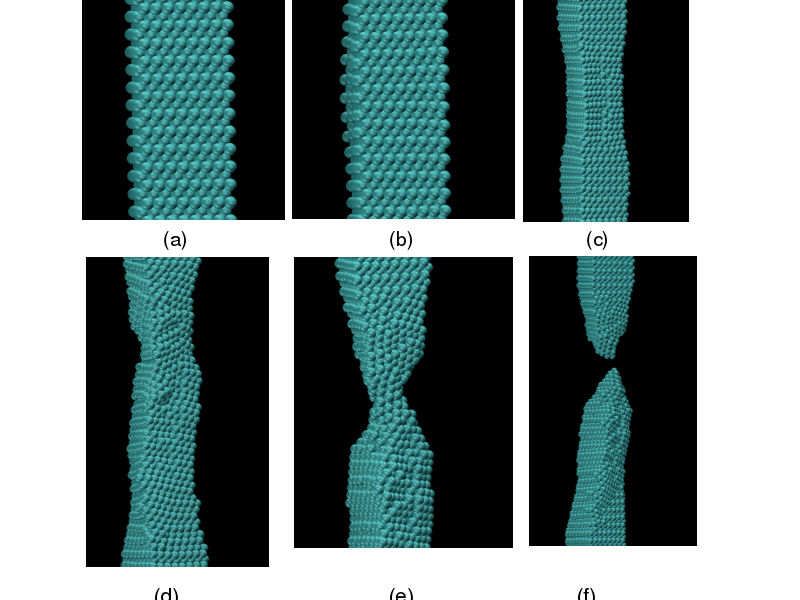
\includegraphics[width=0.6\textwidth]{evolution.png}
            \caption{Stretching evolution of 8x8x36 nanowire.}
        \end{figure}
        % \begin{figure}
        %     \label{fig:correction}
        %     \centering
        %     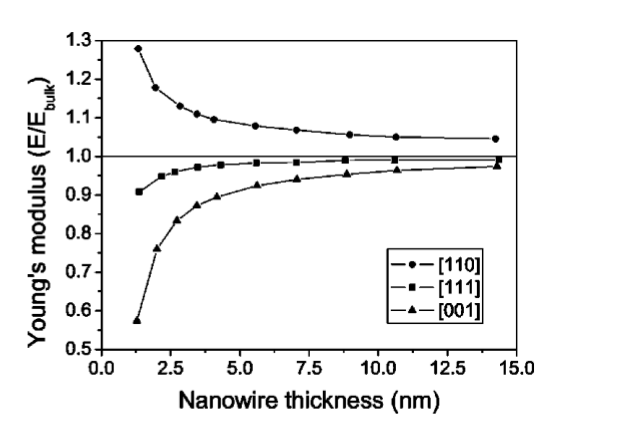
\includegraphics[width=0.6\textwidth]{correction.png}
        %     \caption{Correction factors to relate bulk modulus with MD results.}
        % \end{figure}

        The raw results of the stress tensor are given in ~\ref{fig:rawdata-small} and ~\ref{fig:rawdata-large} for each cross section tested.  The value of interest is the Young's modulus in the direction of displacement.  To obtain this value, the data is taken for $\epsilon_{zz}$ vs $\sigma_{zz}$ over the linear elastic range.  The linear elastic range was visually determined to be the first 5250 and 6750 time steps for the small and large cross sections, respectively.  The Young's Modulus is the slope of the elastic range. Time step (x) is converted to strain, and simulation stress is modified according to 1 (eV/$\AA^3$) = 160 GPa. ~\ref{fig:stress-small-fit} and ~\ref{fig:stress-large-fit} show the fit and Young's Modulus to be 41 and 50 GPA, respectively.  We find that the Youngs modulus is not strongly sensitive to changes in wire aspect ratio, as a doubling of the aspect ratio results in a 20 percent increase in E.  It is of interest to compare this value to that of a macroscopic sample, where $E_{bulk}$ = 117 GPa.  According to \cite{Liang}, the MD calculated Young's Modulus can be compared to the bulk value by considering the thickness of the nanowire.  For the small case, the correction factor of around 0.7 results in a true E = 58.9GPa, leaving a significant discrepancy.

        ~\ref{fig:evolution} shows the behavior of the wire up until fracture. The wire initially carries the strain induced stress without any dislocations in (a).  In (b), the very first visibile dislocations occurs near the center of the wire. (c) begins to show narrowing of the central section of the wire, with buldges propogating towards the ends.   By (d), significant disorder has arisen and out of plane bending is apparent.  (e) exhibits progressive necking to the point of eventual failure, with (f) showing the fracture state and subsequent reduction of stress.  The linear elastic region persists until some point between (c) and (d), when the total bonded cross-sectional area begins to decrease and necking commences.  $\sigma_{z}$ decreases as necking proceeds until reaching approximately zero at fracture.


        \subsection{Collagen Stretching}

        \begin{figure}[!htb]
            \label{fig:coll-evolution}
            \centering
            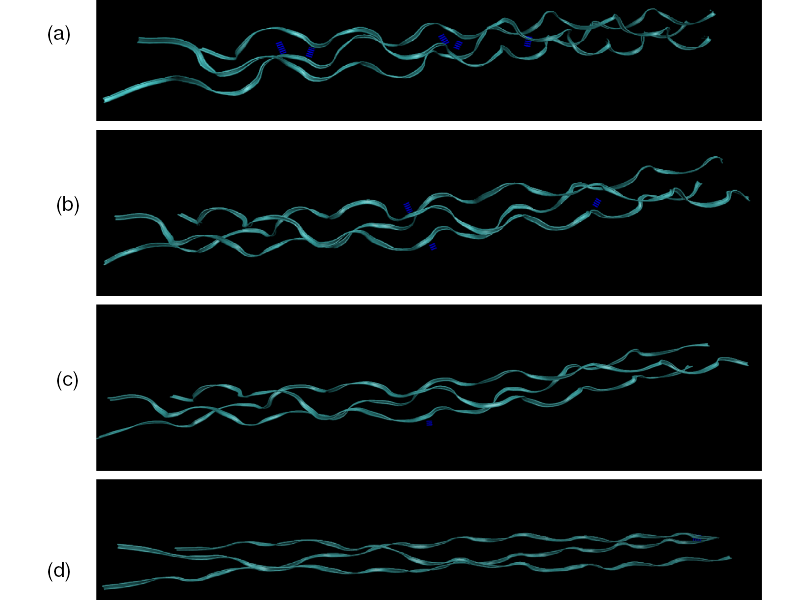
\includegraphics[width=0.6\textwidth]{coll-evol.png}
            \caption{Stretching of collagen molecule.}
        \end{figure}

        \begin{figure}[!htb]
            \label{fig:collagen-young}
            \centering
            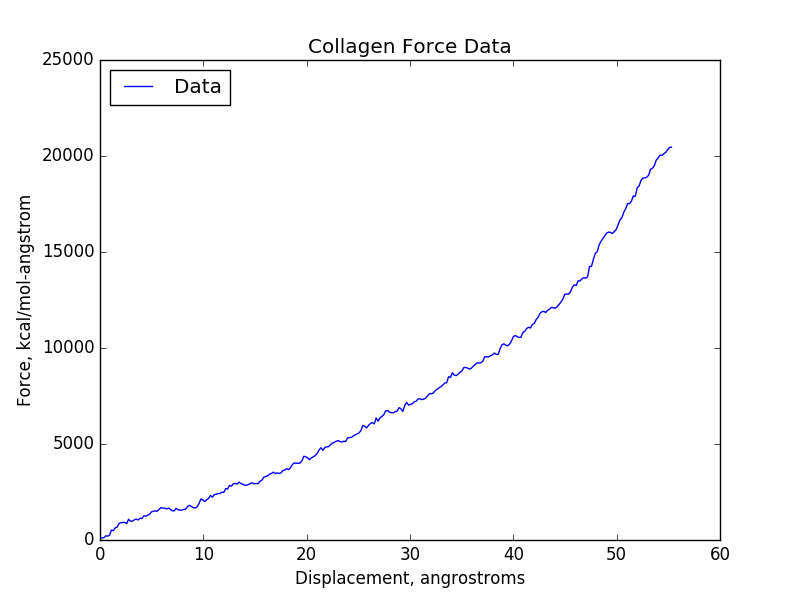
\includegraphics[width=0.6\textwidth]{collagen-stress-strain.png}
            \caption{Force data for collagen stretching.}
        \end{figure}


        Using VMD, the initial length of the molecule was estimated to be 81 $\AA$.  The output log provided information regarding the computation rate, and reported requiring 0.0464128 CPUsec/sim step and 0.537186 CPUdays/ns.  This converts to roughly 1 fs per simulation time step, or 150 ps of total simulation time.  The velocity used was 0.005 $\AA$ / time step (50 m/s).  This at first glance seems high, but considering the velocity of a thermal free neutron at room temperature (2200 m/s), is likely within an order of magnitude of the vibrational "velocity" of collagen.

        From ~\ref{fig:coll-evolution}, we can observe the stretching behavior of collagen.  (a) shows the molecule in its relaxed state, with a handful of hydrogen bonds present.  (b) shows the molecule's initial response to strain, with a slight reduction in hydrogen bond count and the initial unraveling of the strands.  In (c), few hydrogen bonds remain.  (d) shows the molecule almost completely unravelled, but before any major fracture has occured.  It is expected that simulation of further stretching would cause strand failure.

        From ~\ref{fig:collagen-young}, it is found that the Youngs modulus is ~1100 GPa. This does not agree with the value of ~2 GPa for displacements larger than 10 percent \cite{Gautieri}.

        \begin{thebibliography}{5}

        \bibitem{Zhou}
Liang, W., Zhou, M. (2003).Size and Strain Rate Effects in Tensile Deformation of CU Nanowires. 44th AIAA/ASME/ASCE/AHS Structures, Structural Dynamics, and Materials Conference.

        \bibitem{Liang}
        Liang, H., Upmanyu, M.,  Huang, H. (n.d.). Size-dependent elasticity of nanowires: Nonlinear effects. Phys. Rev. B Physical Review B.

        \bibitem{Mohan}
        Mohan R., Liang, Y. Tensile and Flexural Deformation of Nickel Nanowires via Molecular Dynamics Simulations. North Carolina A and T State University. Greensboro, NC, USA.

        \bibitem{Wen}
        Wen, Y., Zhu, Z., Shao, G., Zhu, R. (n.d.). The uniaxial tensile deformation of Ni nanowire: Atomic-scale computer simulations. Physica E: Low-dimensional Systems and Nanostructures, 113-120.

        \bibitem{Gautieri}
        A. Gautieri, et al., Hieracrchical structure and nanomechanics of collagen microfibrilis from the atomistic scale up, Nano Letters, Vol. 11(2), pp. 757-766, 2011.

        \end{thebibliography}



\end{document}
